\documentclass[]{book}
\usepackage{lmodern}
\usepackage{amssymb,amsmath}
\usepackage{ifxetex,ifluatex}
\usepackage{fixltx2e} % provides \textsubscript
\ifnum 0\ifxetex 1\fi\ifluatex 1\fi=0 % if pdftex
  \usepackage[T1]{fontenc}
  \usepackage[utf8]{inputenc}
\else % if luatex or xelatex
  \ifxetex
    \usepackage{mathspec}
  \else
    \usepackage{fontspec}
  \fi
  \defaultfontfeatures{Ligatures=TeX,Scale=MatchLowercase}
\fi
% use upquote if available, for straight quotes in verbatim environments
\IfFileExists{upquote.sty}{\usepackage{upquote}}{}
% use microtype if available
\IfFileExists{microtype.sty}{%
\usepackage[]{microtype}
\UseMicrotypeSet[protrusion]{basicmath} % disable protrusion for tt fonts
}{}
\PassOptionsToPackage{hyphens}{url} % url is loaded by hyperref
\usepackage[unicode=true]{hyperref}
\hypersetup{
            pdfborder={0 0 0},
            breaklinks=true}
\urlstyle{same}  % don't use monospace font for urls
\usepackage[margin=1in]{geometry}
\usepackage{natbib}
\bibliographystyle{plainnat}
\usepackage{color}
\usepackage{fancyvrb}
\newcommand{\VerbBar}{|}
\newcommand{\VERB}{\Verb[commandchars=\\\{\}]}
\DefineVerbatimEnvironment{Highlighting}{Verbatim}{commandchars=\\\{\}}
% Add ',fontsize=\small' for more characters per line
\usepackage{framed}
\definecolor{shadecolor}{RGB}{248,248,248}
\newenvironment{Shaded}{\begin{snugshade}}{\end{snugshade}}
\newcommand{\KeywordTok}[1]{\textcolor[rgb]{0.13,0.29,0.53}{\textbf{#1}}}
\newcommand{\DataTypeTok}[1]{\textcolor[rgb]{0.13,0.29,0.53}{#1}}
\newcommand{\DecValTok}[1]{\textcolor[rgb]{0.00,0.00,0.81}{#1}}
\newcommand{\BaseNTok}[1]{\textcolor[rgb]{0.00,0.00,0.81}{#1}}
\newcommand{\FloatTok}[1]{\textcolor[rgb]{0.00,0.00,0.81}{#1}}
\newcommand{\ConstantTok}[1]{\textcolor[rgb]{0.00,0.00,0.00}{#1}}
\newcommand{\CharTok}[1]{\textcolor[rgb]{0.31,0.60,0.02}{#1}}
\newcommand{\SpecialCharTok}[1]{\textcolor[rgb]{0.00,0.00,0.00}{#1}}
\newcommand{\StringTok}[1]{\textcolor[rgb]{0.31,0.60,0.02}{#1}}
\newcommand{\VerbatimStringTok}[1]{\textcolor[rgb]{0.31,0.60,0.02}{#1}}
\newcommand{\SpecialStringTok}[1]{\textcolor[rgb]{0.31,0.60,0.02}{#1}}
\newcommand{\ImportTok}[1]{#1}
\newcommand{\CommentTok}[1]{\textcolor[rgb]{0.56,0.35,0.01}{\textit{#1}}}
\newcommand{\DocumentationTok}[1]{\textcolor[rgb]{0.56,0.35,0.01}{\textbf{\textit{#1}}}}
\newcommand{\AnnotationTok}[1]{\textcolor[rgb]{0.56,0.35,0.01}{\textbf{\textit{#1}}}}
\newcommand{\CommentVarTok}[1]{\textcolor[rgb]{0.56,0.35,0.01}{\textbf{\textit{#1}}}}
\newcommand{\OtherTok}[1]{\textcolor[rgb]{0.56,0.35,0.01}{#1}}
\newcommand{\FunctionTok}[1]{\textcolor[rgb]{0.00,0.00,0.00}{#1}}
\newcommand{\VariableTok}[1]{\textcolor[rgb]{0.00,0.00,0.00}{#1}}
\newcommand{\ControlFlowTok}[1]{\textcolor[rgb]{0.13,0.29,0.53}{\textbf{#1}}}
\newcommand{\OperatorTok}[1]{\textcolor[rgb]{0.81,0.36,0.00}{\textbf{#1}}}
\newcommand{\BuiltInTok}[1]{#1}
\newcommand{\ExtensionTok}[1]{#1}
\newcommand{\PreprocessorTok}[1]{\textcolor[rgb]{0.56,0.35,0.01}{\textit{#1}}}
\newcommand{\AttributeTok}[1]{\textcolor[rgb]{0.77,0.63,0.00}{#1}}
\newcommand{\RegionMarkerTok}[1]{#1}
\newcommand{\InformationTok}[1]{\textcolor[rgb]{0.56,0.35,0.01}{\textbf{\textit{#1}}}}
\newcommand{\WarningTok}[1]{\textcolor[rgb]{0.56,0.35,0.01}{\textbf{\textit{#1}}}}
\newcommand{\AlertTok}[1]{\textcolor[rgb]{0.94,0.16,0.16}{#1}}
\newcommand{\ErrorTok}[1]{\textcolor[rgb]{0.64,0.00,0.00}{\textbf{#1}}}
\newcommand{\NormalTok}[1]{#1}
\usepackage{longtable,booktabs}
% Fix footnotes in tables (requires footnote package)
\IfFileExists{footnote.sty}{\usepackage{footnote}\makesavenoteenv{long table}}{}
\usepackage{graphicx,grffile}
\makeatletter
\def\maxwidth{\ifdim\Gin@nat@width>\linewidth\linewidth\else\Gin@nat@width\fi}
\def\maxheight{\ifdim\Gin@nat@height>\textheight\textheight\else\Gin@nat@height\fi}
\makeatother
% Scale images if necessary, so that they will not overflow the page
% margins by default, and it is still possible to overwrite the defaults
% using explicit options in \includegraphics[width, height, ...]{}
\setkeys{Gin}{width=\maxwidth,height=\maxheight,keepaspectratio}
\IfFileExists{parskip.sty}{%
\usepackage{parskip}
}{% else
\setlength{\parindent}{0pt}
\setlength{\parskip}{6pt plus 2pt minus 1pt}
}
\setlength{\emergencystretch}{3em}  % prevent overfull lines
\providecommand{\tightlist}{%
  \setlength{\itemsep}{0pt}\setlength{\parskip}{0pt}}
\setcounter{secnumdepth}{5}
% Redefines (sub)paragraphs to behave more like sections
\ifx\paragraph\undefined\else
\let\oldparagraph\paragraph
\renewcommand{\paragraph}[1]{\oldparagraph{#1}\mbox{}}
\fi
\ifx\subparagraph\undefined\else
\let\oldsubparagraph\subparagraph
\renewcommand{\subparagraph}[1]{\oldsubparagraph{#1}\mbox{}}
\fi

% set default figure placement to htbp
\makeatletter
\def\fps@figure{htbp}
\makeatother

\usepackage{booktabs}

\newenvironment{danger}
    {
    \hline\\
    }
    { 
    \\\\\hline
    }
    
\newenvironment{warning}
    {
    \hline\\
    }
    { 
    \\\\\hline
    }
    
\newenvironment{info}
    {
    \hline\\
    }
    { 
    \\\\\hline
    }
    
\newenvironment{try}
    {
    \hline\\
    }
    { 
    \\\\\hline
    }

\author{}
\date{\vspace{-2.5em}}

\begin{document}

{
\setcounter{tocdepth}{2}
\tableofcontents
}
\chapter{Rmarkdown}\label{rmarkdown}

\begin{info}
\emph{Note this is a placeholder page. This material hasn't been taught
yet. I am adding notes online as I can, so these pages in particular may
evolve quickly}
\end{info}

You need to be able to share you analysis. Comments are good for making
code readable, but often you will want longer sections of text, mixed in
with both the code you a running and the outputs of the code (e.g.~the
plots you are making with it). Do this with Rmarkdown.

A Rmarkdown file is a plain text file, like a R script, but with the
extension \texttt{.Rmd} rather than \texttt{.R}. You can make one now in
RStudio by clicking File \textgreater{} New File \textgreater{} R
Markdown. Or by saving an existing .R script as \texttt{filename.Rmd}.

RMarkdown is the system which marks how text should look after it has
been converted into a webpage or PDF or other document. The name
RMarkdown is kind of a joke, since RMarkdown is a verion of a ``markup
langauge''. Markups are the opposite of the
\href{https://en.wikipedia.org/wiki/WYSIWYG}{WYSIWYG} systems (like MS
word or Google Docs) which you are used to.

These pages are written in Rmarkdown. You can see this individual file
\href{https://github.com/tomstafford/psy6422/blob/master/008-rmarkdown.Rmd}{here
in the online repositry}. It will really help if you read the webpage
alongside the file, so you can compare the file which generates the
text, using the markdown, and the output (the webpage).

Rstudio magic (called ``rendering'' or ``knitting'') turns this file in
to the webpage.

Compare the
\href{https://github.com/tomstafford/psy6422/blob/master/008-rmarkdown.Rmd}{file}
and the
\href{https://tomstafford.github.io/psy6422/rmarkdown.html}{webpage}.

\textbf{In the webpage this line is in bold. Why?}

\emph{In the webpage this line is in italic. Why?}

\section{And this line is a heading}\label{and-this-line-is-a-heading}

Try now creating your own Rmarkdown file by clicking File \textgreater{}
New File \textgreater{} Rmarkdown in RStudio.

RMarkdown files have three components.

\section{First a heading}\label{first-a-heading}

That looks like this, at the top of the file

\begin{figure}
\centering
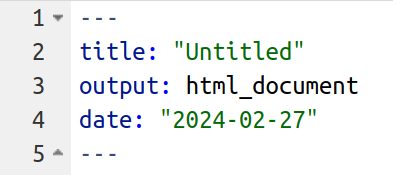
\includegraphics{images/yaml.png}
\caption{Yaml matter at the top of a .Rmd file}
\end{figure}

This is called YAML and it is stuff meant to be read by the computer
when the file is converted into a document to be read by humans. You can
see that this is meant to be an ``HTML'' document (that's the kind on a
webpage), so let's make it now. Click ``knit'' in RStudio (or ``knit to
HTML'' if you are exploring the options menu).

After a brief pause you should get a new window open, containing
something that some of the same words as your document. Notice how the
YAML stuff has disappeared, and the new document now contains formatting
(bold, italics, headings).

Part of the benefit of markdown is that you write the document once, and
can convert it to a webpage, or a PDF, or a MS Word document. Try now.
Click ``Knit'' and select ``Knit to PDF''. It will want you to save the
output file as something (I suggest ``temp.pdf''), but once you've done
that you get a nice PDF document, looking almost, but not entirely, like
the webspage you made moments before.

\section{Second, text}\label{second-text}

If you just write stuff in a \texttt{.Rmd} document you get text. This
is the second kind of thing in a \texttt{.Rmd} document, like this.

It can contain formatting - \emph{italics}, \textbf{bold}, etc - as well
as stuff like lists and hyperlinks:

\begin{itemize}
\tightlist
\item
  See the formatting options in this
  \href{https://github.com/rstudio/cheatsheets/raw/master/rmarkdown-2.0.pdf}{cheatsheet}
\item
  Lists need a second options
\end{itemize}

But the real strength of Rmarkdown is you can mix text and code

\section{Third, code}\label{third-code}

This is the third ingredient. Like this:

\begin{Shaded}
\begin{Highlighting}[]
\KeywordTok{print}\NormalTok{(}\StringTok{"Here is some R code"}\NormalTok{)}
\end{Highlighting}
\end{Shaded}

\begin{verbatim}
## [1] "Here is some R code"
\end{verbatim}

\begin{Shaded}
\begin{Highlighting}[]
\NormalTok{a <-}\StringTok{ }\DecValTok{6}
\NormalTok{b <-}\StringTok{ }\FloatTok{2.3}
\KeywordTok{print}\NormalTok{(a}\OperatorTok{/}\NormalTok{b)}
\end{Highlighting}
\end{Shaded}

\begin{verbatim}
## [1] 2.608696
\end{verbatim}

\begin{Shaded}
\begin{Highlighting}[]
\KeywordTok{print}\NormalTok{(}\StringTok{"And the output it produces"}\NormalTok{)}
\end{Highlighting}
\end{Shaded}

\begin{verbatim}
## [1] "And the output it produces"
\end{verbatim}

Here is another example

\begin{Shaded}
\begin{Highlighting}[]
\CommentTok{#Code to make an example graph}
\KeywordTok{library}\NormalTok{(tidyverse)}

\CommentTok{#load some data}
\NormalTok{filename <-}\StringTok{ '/home/tom/Desktop/psy6422/mydatafile.csv'}
\NormalTok{df <-}\StringTok{ }\KeywordTok{read.csv}\NormalTok{(filename)}

\CommentTok{#rename columns for easy labelling}
\NormalTok{df <-}\StringTok{ }\NormalTok{df }\OperatorTok\StringTok{ }\KeywordTok{rename}\NormalTok{(}\DataTypeTok{ppt =}\NormalTok{ Participant.Number,}\DataTypeTok{asrs =}\NormalTok{ Total.ASRS.Score)}

\CommentTok{#plot parameters}
\NormalTok{plottitle  <-}\StringTok{  'ASRS values for each participant'}
\NormalTok{xlab  <-}\StringTok{  'Participant number'}
\NormalTok{ylab  <-}\StringTok{  'Total ASRS score'}
\NormalTok{pointsize  <-}\StringTok{  }\DecValTok{7}

\CommentTok{#make plot}
\NormalTok{p1 <-}\StringTok{ }\KeywordTok{ggplot}\NormalTok{(}\DataTypeTok{data=}\NormalTok{df,}\KeywordTok{aes}\NormalTok{(}\DataTypeTok{x=}\NormalTok{ppt,}\DataTypeTok{y=}\NormalTok{asrs))}
\NormalTok{p1 }\OperatorTok{+}\StringTok{ }\KeywordTok{geom_point}\NormalTok{(}\DataTypeTok{size=}\NormalTok{pointsize) }\OperatorTok{+}
\StringTok{  }\KeywordTok{ggtitle}\NormalTok{(plottitle) }\OperatorTok{+}
\StringTok{  }\KeywordTok{xlab}\NormalTok{(xlab) }\OperatorTok{+}
\StringTok{  }\KeywordTok{ylab}\NormalTok{(ylab)}
\end{Highlighting}
\end{Shaded}

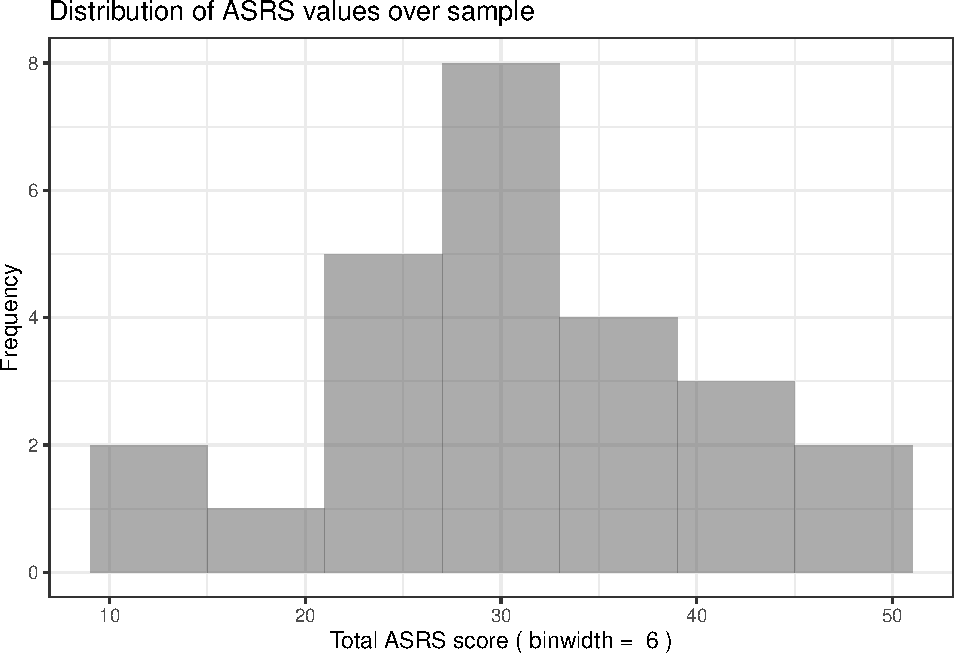
\includegraphics{008-rmarkdown_files/figure-latex/unnamed-chunk-3-1.pdf}

You don't need to show the r code, but still include it in the document
and use it to generate figures etc.

The scatterplot above uses participant number as one of the axes, which
doesn't really make any sense. A histogram is a better way of
visualising the spread of scores on a single variable, so here is one:

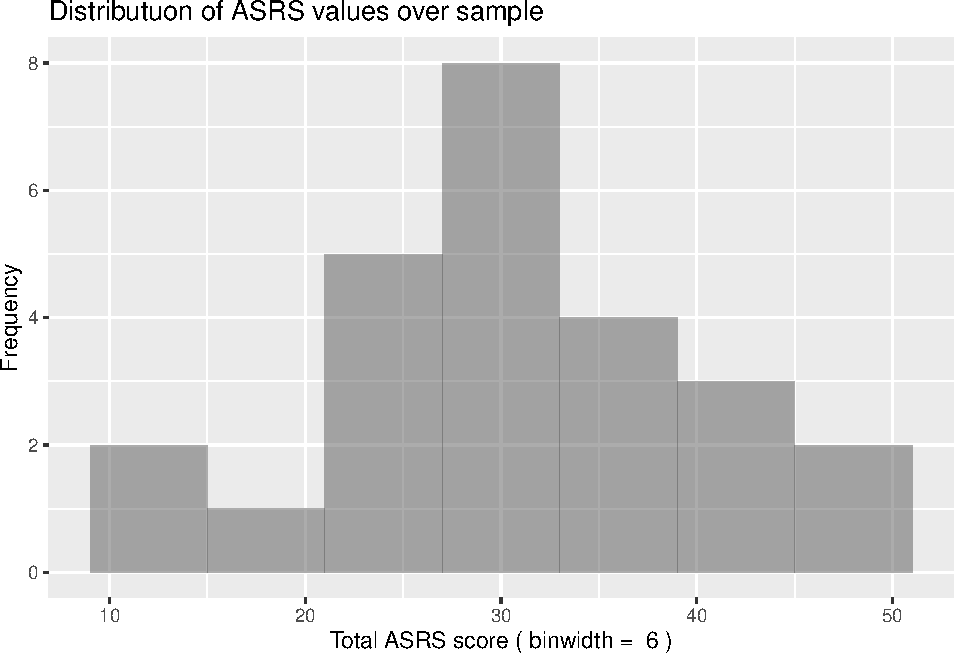
\includegraphics{008-rmarkdown_files/figure-latex/unnamed-chunk-4-1.pdf}

The code to make this plot is contained in the same \texttt{.Rmd} file
as this text, but I've hidden it so only the output is shown. To do this
I set
\texttt{echo\ =\ FALSE\textquotesingle{}\textquotesingle{}\ for\ the\ r\ chunk\ in\ the}.Rmd``
file. You'll have to look at the
\href{https://github.com/tomstafford/psy6422/blob/master/008-rmarkdown.Rmd}{source
file} to see this, because - obviously! - in the webpage you don't see
any code.

\section{Conclusion}\label{conclusion}

\section{Exercises}\label{exercises}

\section{Resources}\label{resources}

\begin{itemize}
\tightlist
\item
  \href{https://rmarkdown.rstudio.com/}{RStudio intro to Rmarkdown}
\item
  \href{https://github.com/rstudio/cheatsheets/raw/master/rmarkdown-2.0.pdf}{RStudio
  RMarkdown cheatsheet}
\end{itemize}

\end{document}
